\documentclass[APA,STIX1COL]{WileyNJD-v2} %AMA,
\usepackage{moreverb}

\setcitestyle{aysep={,}, yysep={;}} %Citation-related commands

%zur Einbindung von Graphiken
\usepackage{graphicx}
%Bearbeitung von Kopf- und Fusszeile
\usepackage{fancyhdr}
%Schriftart
\usepackage{helvet}
%stellt unabhängige Textmarken zu Verfügung
\usepackage{extramarks}
%aktiviert eine Umgebung in der der Mathematikmodus aktiv ist
\usepackage{amsmath}
%coole Zeichentools
\usepackage{tikz}
\usetikzlibrary{arrows.meta}
%aktiviert eine Umgebung in der der Mathematikmodus aktiv ist
\usepackage{amsthm}
%aktiviert eine Umgebung in der der Mathematikmodus aktiv ist
\usepackage{amssymb}
%Mehrzeilige Tabellen
\usepackage{tabularx}
\usepackage{multirow}
\usepackage{booktabs}
%For algorithms
\usepackage{algorithm}
\usepackage{algpseudocode} % [noend]notwendig? wirft fehler -> sonst Param global uebergeben
%Für Subfigures
%\usepackage{caption} 
\usepackage{subcaption}
%Stellt das Eurozeichen ? zu Verfügung
\usepackage[right]{eurosym}
    % package to open file containing variables
    \usepackage{datatool, filecontents}
    \DTLsetseparator{ = }% Set the separator between the columns.
    
\def\blankpage{%
      \clearpage%
      \thispagestyle{empty}%
      \addtocounter{page}{-1}%
      \null%
      \clearpage}

\usepackage{placeins} 
%\usepackage[colorinlistoftodos,prependcaption,textsize=tiny,disable]{todonotes}

\usepackage[utf8]{inputenc} 		% Nur einbinden, wenn LuaLatex nicht vorhanden!
%\usepackage[ngerman, english]{babel} %  Wirft Fehler
\usepackage[T1]{fontenc}


\usepackage[acronyms,ucmark=true]{glossaries}
\makenoidxglossaries



\usepackage{fancybox}
\usepackage{xcolor}
\usepackage{color}
\usepackage{float}
\usepackage{framed}
%\usepackage{url}
%\usepackage{newclude} %breaks APA citation style
\usepackage{diagbox}
%aktiviert Hyperlinks
\hypersetup{
  hidelinks
}
\usepackage{hyperref} 


\newcommand\BibTeX{{\rmfamily B\kern-.05em \textsc{i\kern-.025em b}\kern-.08em
T\kern-.1667em\lower.7ex\hbox{E}\kern-.125emX}}

\articletype{Research Article} % Article Type}%

\received{<day> <Month>, <year>}
\revised{<day> <Month>, <year>}
\accepted{<day> <Month>, <year>}

%\raggedbottom

\begin{document}

\title{Benefits of International Collaboration in Computer Science: A Case Study of China, the European Union, and the United States}

\author[1]{Alberto Gómez-Espés*}

\author[2]{Adam Jatowt}

\author[3]{Michael Färber}

\authormark{GÓMEZ-ESPÉS \textsc{et al}}


%\address[2]{\orgdiv{Org Division}, \orgname{Org name}, \orgaddress{\state{State name}, \country{Country name}}}

\address[1]{\orgdiv{Department of Information Systems, Production and Logistics Management}, \orgname{University of Innsbruck}, \orgaddress{\state{Tirol}, \country{Austria}}}

\address[2]{\orgdiv{Department of Computer Science}, \orgname{University of Innsbruck}, \orgaddress{\state{Tirol}, \country{Austria}}}

\address[3]{\orgdiv{Institute AIFB}, \orgname{Karlsruhe Institute of Technology (KIT)}, \orgaddress{\state{Baden Württemberg}, \country{Germany}}}

\corres{*Corresponding author name, Corresponding address. \email{Alberto.Gomez-Espes@student.uibk.ac.at}}

\presentaddress{Innrain 52, 6020 Innsbruck, Austria}

\abstract[Abstract]{Co-authored publications can bring positive results for those who participated, such as accessing more funding or increasing the publication impact. China, the European Union, and the United States have been collaborating between them throughout the years in the field of Computer Science. These collaborations have been varying over time, as well as they have impacted the regions in different ways. In this paper, we obtained the publications from these territories across 31 years on the topic of Computer Science and studied them focusing on how the regions have approached co-authorship. In particular, we have analyzed the number of collaborations during that period, the impact of those papers measured as number of citations, and the topics that have been studied in those associations. We have concluded that China’s focus on STEM has led it to be the most productive region in recent years; plus, it has benefited from the US and European impact. On the other hand, the EU and the US have benefited from Chinese funding and workload, increasing the number of publications together.}

\keywords{computer science, co-authorship, collaboration, citation}

\jnlcitation{
%\cname{%
%\author{Williams K.}, 
%\author{G. Masato}, and 
%\author{T. Woollings}} (\cyear{2016}), 
%\ctitle{A regime analysis of Atlantic winter jet variability applied to evaluate HadGEM3-GC2}, \cjournal{Q.J.R. Meteorol. Soc.}, \cvol{2017;00:1--6}. 
}

\maketitle


\section{Introduction}
\label{sec:introduction}

The proportion of internationally co-authored scientific papers has significantly increased since the turn of the century, representing a growing share of all scientific cooperation, while in-home collaboration has been falling \citep{adams2013fourth, choi2015quantifying,wagner2015continuing}.

This growth is mainly attributed to the participation of scientifically advanced countries such as the US or some of the countries in the European Union, with scientific emerging countries such as China also increasing their involvement through increased spending on research and development, resulting in their increased appearance as partners in internationally co-authored scientific papers \cite{wagner2015continuing}.
International collaboration can bring positive results in general to the countries that participated in it. For example, papers co-authored by individuals from multiple nations receive higher citation rates compared to those authored by individuals from a single nation \citep{levitt2010does,glanzel2001double,kwiek2021globalization}. Another positive trend observed is that co-authored publications receive higher citation rates compared to single-authored papers \citep{ronda2022immediacy, shen2021correlation}. But apart from general benefits, international coauthoring can also bring specific advantages for a country depending on the other countries it is collaborating with, such as access to more funding opportunities, more R\&D activity, and local knowledge \citep{lee2020winners,harhoff2014channels}.
The top 3 most scientific works producers are China, the European Union (EU), and the United States (US), also they are their major collaborators, as well as the ones that received more citations \citep{wang2017network,zhang2018china, burke2022state}. Although the scientific collaborations between China and the US have been increasing during previous decades, recent studies suggest that this tendency has stopped \citep{schuller2020united,cai2021international,lacey2021technological,zhao2019technology}. This rivalry leaves the EU in the middle of a crossfire, in which it is not clear yet if it will follow the anti-China approach proposed by the US or will follow another path keeping the positive collaboration tendency \citep{schuller2020united,ullah2020eu}. It is in this context that we want to contribute to the current literature by providing a long-term analysis of these territories.
In this paper, we examine the collaboration tendencies between China, the US, and the UE during 31 years in the field of computer science, observing the impact on publications considering the aim of the institutions that work on the co-authorship. Therefore, we contribute to the current literature in 3 ways.  First, we conduct an analysis of how the regions have been collaborating between them over time, as well as providing insights based on the type of institutions that collaborated. Second, we investigate the impact of those collaborations on the article’s outcomes in both academic and privately owned papers. Third, we analyze how the different countries have been prioritizing the different fields of computer science over time, and how they have been sharing their interest between them.

The subsequent sections of this paper are organized as follows: In Section~\ref{sec:related_work} we discuss related work of research collaborations, as well as provide current literature about the relations between China, the EU, and the US in scientific co-authorship. In Section~\ref{sec:data_set}, we provide the details about our dataset and explain the process we followed to collect and analyze it. Section \ref{sec:results} shows the results we obtained when investigating the data. Finally, draw a conclusion with the findings we got and outline potential future research in Section~\ref{sec:conclusion}.
%\section{Fundamentals}
\label{sec:fundamentals} 
\section{Related Work}
\label{sec:related_work}

\subsection{Scientific copublication}

Publication co-authorship has been thoroughly examined within the field of bibliometrics, which is a quantitative branch of information and library science that studies the publication of research accomplishments \citep{broadus1987toward}. Different studies suggest that collaborating can bring different advantages, such as higher productivity, higher impact, and higher quality. However, it may also bring about certain drawbacks, such as a potential lack of comprehension and cohesion between collaborators, as well as the potential for disputes over authorship credit \citep{besancenot2017co,franceschet2010effect,biscaro2014co}. Despite the possible disadvantages, cooperation in research continues to grow in most academic disciplines \citep{wagner2015recent,wagner2017growth,chinchilla2019follow}. However, this tendency, as well as the collaboration outcomes, might vary within disciplines and whether the collaboration has been national or international \citep{franceschet2010effect,puuska2014international}.
Focusing on collaboration within the different areas of science, previous literature suggests that international collaborations have been increasing in recent years, as measured by the number of co-authored papers, with global collaboration continuing to grow as a share of all scientific cooperation \citep{lariviere2013bibliometrics}. Different studies have examined the citation impact of international and domestic co-publishing in different scientific disciplines, and they have found that international collaboration has a higher citation impact than domestic collaboration in sciences \citep{puuska2014international,lancho2010lies,newman2004coauthorship}. Finally, in the field of computer science, it has been also found that its research networks are widely connected, allowing new collaborations to be created between scientists from different institutes, countries, or sub-disciplines \citep{franceschet2011collaboration}.

\subsection{Chinese - American collaborations}
The United States and China have been the two leading countries in global research and development (R\&D) performance during the last decades \citep{burke2022state}. Although the number of collaborations between these countries, measured as the number of scientific papers co-published, has constantly increased, their positioning is as global adversaries instead of allies \citep{wagner2015recent,lee2020winners,zhao2022one,lewis2021time}. This can be seen in recent findings suggesting that the collaboration between these countries has been slightly decreasing, even when the relationship between the two countries can bring advantages to both \citep{wagner2022changes,wagner2022drop,cai2021international}. Previous studies suggest that the collaborations between the US and China bring more citations than only those authored by Chinese researchers \citep{tang2011china}. On the other hand, the US benefit from collaborating with China by obtaining funds for research, as well as increasing their scholarly output \citep{lee2020winners}.

\subsection{European - American collaborations}

Although the global concentration of R\&D performance continues shifting from the United States and Europe to countries in East-Southeast Asia and South Asia, scientific publications made by the EU and the US are more relevant than those that these regions published collaborating with China \citep{leydesdorff2014european, burke2022state}. Apart from this higher impact, the US and the EU benefit from each other’s specializations in the different scientific fields \citep{burke2022state}. In addition to this, European countries have also benefited from the rivalry between China and the US, attracting more collaborations between the US and the EU \citep{schuller2020united,wagner2022drop,cai2021international}.

\subsection{Chinese - European collaborations}

The EU and China are the countries where more Science and Engineering articles are produced respectively \citep{burke2022state}. In recent years, the collaboration between them has grown fast, turning the European Union into the second biggest partner of China in science and technology research \citep{li2014beyond}. This collaboration tendency between the EU and China varies among the EU former countries. However, it represents more than 20\% of total Chinese collaborations \citep{wang2017network,yuan2018international}. Previous findings indicate that the proportion of Chinese scientists living abroad is significantly higher in the USA compared to the EU. However, the flow of researchers from these destinations coming back to China has been more pronounced from the EU than the USA, which can increase international collaboration with their previous locations \citep{cao2020returning}. That trend, summed with political reasons can be the cause of that Chinese researchers still want to collaborate with EU institutions instead of US institutions \citep{schuller2020united,silver2020us,wagner2022drop}.

\section{Data Set}
\label{sec:data_set}

\subsection{Dataset}

For our analysis, we used OpenAlex as data source, a fully open scientific knowledge graph (SKG) that replaces the previously discontinued Microsoft Academic Graph (MAG) \citep{priem2022openalex}. On 15th of April of 2023, the OpenAlex dataset had 245M works, which include journal articles, books, datasets, and theses. OpenAlex allows using filters in advance, setting thresholds to the search, and therefore reducing the processing time.

\subsection{Data collection}

In the following section, we discuss the process we followed for the data collection. 

We gathered information on the works by utilizing OpenAlex API, using various filters. First, we filtered works by the “computer science” concept, considering only journal articles, and limiting the publication year from 1990 to 2021, both inclusive. In addition to this, we filtered retracted publications.

\subsection{Data preprocessing}

Before starting to work with the data, we had to pre-process the raw data. As the scope of this research paper is to analyze the collaboration patterns between different countries and regions, papers written by just one author were removed, and we only considered publications whose all authors were affiliated with an educational or company institution. There were works that did not have their DOI code attached, nor either the number of citations that were also removed. To categorize the publications, we added a tag to mark each work based on the institutions’ type that participated in the collaboration. Therefore, works where all participants were affiliated with educational institutions, such as universities, were categorized as “educational”, works where all participants came from profit-oriented private corporations were categorized as “company”, and those works done by both were marked as “mixed”. In this experiment, we considered EU publications published by the EU27 as well as the UK to simplify, and China publications published by “China Mainland”. It resulted in a dataset composed of 2.443.196 research papers.
%\section{Diversity Framework} % {Methodology}
\label{sec:methodology}

To investigate the mixture and diversity of topics of news articles, we first extract the topics from the headlines. This is a text mining and natural language processing task, usually based on topic modeling in existing works. 
% Given a corpus of documents, in our case the headlines, topic modeling identifies underlying topics in these documents. 
Having the allocation between headlines and topics, we can investigate the diversity of the result sets.

\subsection{Topic Modeling}

Topic modeling is based on the assumption that documents are composed of one or more topics. We used two topic modeling methods to see which performs superior on our data set. The first one being 
% the state-of-the art probabilistic topic model, LDA.
the widely used Latent Dirichlet Allocation (LDA). Existing literature pointed out that LDA perform weak on shorter texts (even when optimized) as there is little word co-occurrence information \citep{lin_dual-sparse_2014, qiang_short_2020, li_enhancing_2017}. Furthermore, LDA assumes that there are multiple topics in a document, which might not be true for headlines. 
Considering only headlines, our documents are very short, namely in the case of the Top Stories data set on average \var{title_length_avg} words with a standard deviation of \var{title_length_std}. 
% Usually LDA documents are longer. 
The authors of the survey \citet{qiang_short_2020} 
% created a survey on Short Text Topic Modelling. In their study they 
identified GPU-PDMM as best algorithm for their Google News data set with the highest classification accuracy \citep{qiang_short_2020}. We therefore use this method as second one for our work. 

GPU-PDMM is a Poisson-based Dirichlet Multinomial Mixture model (PDMM) 
with a generalized Pólya urn (GPU) model. 
Despite its reliance on a Poisson-based model, each document consists of only a few topics \citep{qiang_short_2020}.  Using the GPU-model, additional external knowledge about word semantics can be used to improve topic modelling, especially with short texts \citep{li_enhancing_2017}. This paper will build on \citet{qiang_short_2020}'s result and use a JAVA implementation\footnote{\href{https://github.com/qiang2100/STTM}{https://github.com/qiang2100/STTM} (Last accessed 01/03/2022)} of GPU-PDMM and LDA provided by \citet{qiang_short_2020}.


%\subsubsection
\textbf{Preparing Data Set for Topic Modeling.}
To identify the topics in the overall news as accurately as possible, we 
% provide it 
consider 
not only the data gathered from Google Top Stories, but also from Google News and Bing News. 
% Therefore, our used corpus are the headlines from all three, our control data set.

To run topic modeling, the headlines 
% need to be preprocessed. 
% In the preprocessing described in \textit{\ref{subsec:data_preprocessing} \nameref{subsec:data_preprocessing}}, additional pre- and suffixes were already deleted. The goal of preprocessing is to reduce the complexity of the documents. Here, the following state-of-the-art steps were performed: 
% For preprocessing, we perform the following steps: 
are preprocessed, including (i)~the removal of special characters, (ii)~lower casing text, (iii)~lower casing text, (iv)~tokenization of text, (v)~lemmatizing, (vi)~the removal of rare words (with fewer than 3 occurrences), and (vii)~the removal of words with little context.


%\subsubsection
\textbf{Running Topic Modeling on our Data Set. }
\label{subsec:running_topicmodelling}
%
As we are using only two different topic modeling approaches using the default values (except the number of iterations for GPU-PDMM, as GPU-PDMM performs well even with little iterations \citep{qiang_short_2020}), this yields an open question of further optimizing the topic modelling. 
The $\alpha$ and $\beta$ hyperparameters of our approaches are based on defaults used in the literature\footnote{\url{https://github.com/qiang2100/STTM}}. All used parameters are noted in Table \textit{\ref{table:topic_modelling_parameters}}.

%\input{tables/topic_modelling_parameters}
\begin{table}[tb]
\centering
\begin{tabular}{lcc}
\toprule 
    & \textbf{LDA }
    & \textbf{GPU-PDMM}
\\ 
\midrule
    Number of topics    
    & 3-50
    & 3-50
\\
    Number of iterations    
    & 1000
    & 48
\\
    $\alpha$ hyperparameter     
    & 0.1
    & 0.1
\\
    $\beta$ hyperparameter
    & 0.01
    & 0.01
\\
\bottomrule
\end{tabular}
\caption{Topic modelling parameters}
\label{table:topic_modelling_parameters}
\end{table}

To select the optimal amount of topics, we run topic modeling multiple times with each iteration having a different setting for the number of topics, ranging from 3 to 50 topics. 
The final amount of topics is then determined by comparing the coherence scores per setting and selecting the maximum. 
For this task, we used the built-in function of the STTM framework \citep{qiang_short_2020}. 
%% It builds on the PMI, calculating the likelihood of co-occurrence of words in a sliding 10-word window based on a dump of the German Wikipedia.\footnote{\url{https://dumps.wikimedia.org/dewiki/20211020/dewiki-20211020-pages-meta-current.xml.bz2}} 

Figure \textit{\ref{fig:coherence_scores}} shows the identified coherence scores for both LDA and GPU-PDMM on our data set. The maximum coherence score in our example was 0.3566 using GPU-PDMM and \var{number_of_topics} topics, and was therefore used. We see, in general, that GPU-PDMM performs better on our data set, looking at the coherence scores. With a high number of topics, the topics get so fine-grained that the differences are not that large any more. 
Running the topic modeling on this corpus and optimizing topic coherence scores, we find \var{number_of_topics} topics as the best in our case. For the full list of all identified topics and its related top 20 words, we can refer to our repository. 
% Table \textit{\ref{table:identified_topics}}. 

\begin{figure}[tb]
    \centering
    \includegraphics[width=0.6\textwidth]{images/topic_coherence_graph.png}
    \caption{Coherence scores}
    \label{fig:coherence_scores}
\end{figure}


%\subsubsection
\textbf{Document-Topic Assignment. }
%
To analyze the topic diversity of headlines, we need an assignment of a topic for a headline. We introduce a notation for this headline-topic assignment:
$t(h): Headline \rightarrow Topic$. For instance, the topic of headline $h_1$ would be: $t(h_1) = t_5$.

After preprocessing our headlines, we use the transformed headlines from Section \ref{subsec:data_preprocessing} as an input for our topic modeling. 
%Figure \textit{\ref{fig:document_topic_assigment_example}} shows such an exemplary preprocessing.

%\begin{figure}[tb]
%    \centering
%    \includegraphics[width=0.8\textwidth]{images/document-topic-assigment-example.png}
%    \caption{Example of original and preprocessed headline}
%    \label{fig:document_topic_assigment_example}
%\end{figure}

%\begin{minipage}{\textwidth}

    The used STTM framework then provides different outputs in the form of 
    \begin{itemize}
        \item \textbf{document-to-topic distributions}: Each headline has a probability distribution over all topics. $t(h)$ is then the topic with the highest probability. If two topics have the same probability, $t(h)$ is the topic with the lower index. 
        
        \item \textbf{topic assignment}: Each word in the headline is connected to one topic. $t(h)$ is the topic appearing the most. If two topics occur the same number of times, we define $t(h)$ as the topic with the lower index. 
    \end{itemize}

%    \vspace{2mm} 
%\end{minipage}



\subsection{Measuring Topic Diversity} %  of the Data Set
\label{subsec:methodology_data_set_diversity}

In this section we discuss how the dimensions variety, balance and disparity apply on the level of the whole data set. Section \ref{subsec:methodology_result_set_diversity} then discusses how these dimensions apply to the result sets of the searches. Whilst Section \ref{subsec:methodology_data_set_diversity} and \ref{subsec:methodology_result_set_diversity} discuss these applications in theory, Section \ref{sec:results} applies this to the Google Top Stories federal election data set.

\subsubsection{Variety} %  of the Data Set
\label{subsec:methodology_data_set_diversity_variety}
Variety gives information about how many categories occur \citep{macarthur_patterns_1965}, in our case counting all unique topics. 
As the topic model takes the number of topics as an input and then outputs exactly this amount of topics, the variety is exactly the number of topics in topic modeling. As one can create the value of variety ``manually'', looking at variety would only make sense comparing subsets of the data set. 
One could, for instance, investigate in the number of topics per search query. 
Another example will be discussed in Section \ref{subsec:methodology_result_set_diversity}, looking into the structure and diversity of result sets (which then of course could also be aggregated again into result set diversity per query or query category).

\subsubsection{Balance} %  of the Data Set
\label{subsec:methodology_data_set_diversity_balance}
The balance of the overall topics of the data set would be how many headlines are assigned to each topic. How a distribution should look in order to be considered diverse in terms of balance differs according to the underlying normative frameworks.
We argue that in the deliberative normative framework, this would be a uniform distribution or at least a distribution similar to it \citep{loecherbach_unified_2020}. Thus, every topic has the same or at least a similar amount of assigned headlines. Consequently, all viewpoints, entities and in this case topics, should be represented equally in the news debate.

To bring the theoretical concept of balance into a measurable variable, we use 
Shannon's Evenness index (SEI) \citep{loecherbach_unified_2020}. 
% SEI. 
Originating from diversity of biotopes in biology, SEI has found broad adaption in different research disciplines \citep{van_dam_diversity_2019}. 
The SEI of a result set $X$ is calculated by dividing the Shannon Diversity Index (SDI) of $X$ by its maximum:
% \footnote{\url{https://en.wikipedia.org/wiki/Species_evenness}}

\[SEI(X) = \frac{SDI}{max(SDI)} = \frac{SDI}{ln(|X|)} = \frac{-\sum_{i}^{|X|}(p_i * ln(p_i))}{ln(|X|)} \in [0,1]\]

with $p_i$ being the proportion of articles that belongs to the topic currently iterated over. The higher the SEI value, the more uniform a distribution is.


\subsubsection{Disparity} %  of the Data Set
\label{subsec:methodology_data_set_diversity_disparity}

In contrast to variety and balance where it is only important that different topics are distinct, disparity measures how similar and therefore also different the topics are semantically. 

Our approach is as follows: We use the generated top words from topic modeling to calculate a numerical representation of each topic. For each top word, we get the word embedding of a representation. The average of all top word embeddings then represents the embedding for the overall topic. To get the similarity between different topics, we use the cosine-similarities between every topic. The correlation between these two sizes is $Disparity = 1 - Similarity$. A similarity value of 1 means that the two topics are identical, and lower weights meaning less similarity. The other way around, a disparity value of 0 means that the two topics are identical and higher values meaning higher disparity. 
These values could be represented by “disparity weights” on weighted edges of a complete graph $G = (V, E)$ with $V = t_0, ..., t_n$ and $E = \{\{t_i, t_j\}: 0 \leq i \leq j \leq n\}$ the respective weights $w: E \rightarrow \mathbb{R}$. Figure \textit{\ref{subfig:disparity_weighted_graph_disparity}} illustrates this in an example.

% This approach also opens the field for potential further research and quantification, using some more data for distinguishing the topics (e.g., using knowledge graphs).

\begin{figure}[tb]
    \centering
    \begin{subfigure}{.3\textwidth}
        \centering
        \includegraphics[width=\textwidth]{images/disparity_example_weighted_graph_disparity.png}
        \caption{Example disparity graph}
        \label{subfig:disparity_weighted_graph_disparity}
    \end{subfigure}
    \begin{subfigure}{.3\textwidth}
        \centering
        \includegraphics[width=\textwidth]{images/disparity_example_weighted_graph_similarity.png}
        \caption{Corresponding similarity graph}
        \label{subfig:disparity_weighted_graph_similarity}
    \end{subfigure}
    \caption{Relationship between disparity and similarity graph}
    \label{fig:disparity_weighted_graph}
\end{figure}

Disparity for the full data set would mean looking into how distinct and different from each other the identified topics are. Motivated on a simple example, this would, for instance, mean that the two topics ``football'' and ``finance'' have a higher disparity (=lower similarity) than for example ``football'' and ``athletes''. By quantifying these ``distances'', one can better understand how similar or different two search results are by comparing all the topics against each other.


% Theory for d
% Methods for 
\subsection{Determining Topic Diversity of Result Sets}
\label{subsec:methodology_result_set_diversity}

The following section discusses the same dimensions as in Section \ref{subsec:methodology_data_set_diversity}, but now on the level of result sets. For the Section \ref{sec:results}, the respective values are calculated for each result set and then aggregated into one overview.

\subsubsection{Variety of Result Sets} In the following let $V(X)$ denote the variety of a result set $X$. The basic intuition behind variety is ``the more, the better''. In the case of topic diversity, that would be: The more topics covered by a result set, the better. 

Limited only through the overall data set variety (i.e., not considering the number of results), the following applies to the variety $V$ of a result set $S$:
\[
    0 \leq V(S) \leq \var{number_of_topics} \text{ with } V(S) \in \mathbb{N}_0\text{.}
\]


% As we only consider one topic per headline, determining the variety is rather straightforward. 
To determine the variety of a result set, one has to count all unique topics. 
As each result set has a maximum of 10 results in our case and each result has exactly one topic, the variety of this result set is exactly the number of unique topics. Considering only one topic per headline and the maximum amount of 10 results per result set, we can restrict above condition further to
\[
    0 \leq V(S) \leq 10 \text{ with } V(S) \in \mathbb{N}_0\text{.}
\]
A variety of 10 would mean that every result in the result set has a different topic.

In the example in Figure \textit{\ref{fig:variety_absolute_topic_difference}}, result set $A$ is – only related to variety – more diverse than $B$, as it has 3 instead of only 2 unique topics. 
That might be unintuitive at first glance, as result set $B$ has more results than $A$.

\begin{figure}[tb]
    \centering
    \includegraphics[width=\textwidth]{images/variety_absolute_topic_difference.png}
    
   % \begin{table}[tb]
    %    \centering
        \begin{tabularx}{\textwidth}{XXXl}
        \toprule 
        & \textbf{Result set $A$} & \textbf{Result set $B$} & \textbf{Diversity} \\
        \midrule
        \textbf{Absolute topics} & $|\{t_1, t_2, t_3\}| = 3$ & $|\{t_1, t_2\}| = 2$ & $V(A)=3 > V(B)=2$ \\
        \bottomrule
        \end{tabularx}
    %\end{table}
    
    \caption{Simple example for variety with one topic}
    \label{fig:variety_absolute_topic_difference}
\end{figure}

Variety in itself is not sufficient to determine diversity, although it is often used as such. The approach of using variety as a measure for diversity is often used on source diversity, where researchers argue that higher source variety (so the more news sources) the better the diversity. This has been critiqued by multiple researchers (e.g., \citet{carpenter_study_2010,napoli_deconstructing_1999}).


\subsubsection{Balance of Result Sets}

Building on variety, which only take into account the absolute number of topics, balance now looks at how the topics are distributed across the headlines. 
In most cases, a result set would be considered diverse, if the distribution of the topics are somehow equal or even (discrete uniform distribution). 
An extreme example with a low diversity would be a result set with 10 results, of which 8 are about the same topic and the other both another one. This could be considered having a low balance. 


Coming back to the example in Figure \textit{\ref{fig:variety_absolute_topic_difference}}, we would have the distribution illustrated in Figure \textit{\ref{subfig:balance_example_actual}}, although a more even distribution like Figure \textit{\ref{subfig:balance_example_optimal}} would be preferred.

\begin{figure}[tb]
    \centering
    \begin{subfigure}{\textwidth}
        \centering
        \includegraphics[width=0.55\textwidth]{images/balance_example_visual.png}
        \caption{Alternative visualization of result set B in Figure \ref{fig:variety_absolute_topic_difference}}
        \label{subfig:balance_example_visual}
    \end{subfigure}
    \begin{subfigure}{.3\textwidth}
        \centering
        \includegraphics[width=0.6\textwidth]{images/balance_example_actual.png}
        \caption{Actual balance}
        \label{subfig:balance_example_actual}
    \end{subfigure}
    \begin{subfigure}{.3\textwidth}
        \centering
        \includegraphics[width=0.6\textwidth]{images/balance_example_optimal.png}
        \caption{Optimal balance}
        \label{subfig:balance_example_optimal}
    \end{subfigure}
    \begin{subfigure}{.3\textwidth}
        \centering
        \includegraphics[width=0.6\textwidth]{images/balance_example_optimal_2.png}
        \caption{Alt. optimal balance}
        \label{subfig:balance_example_optimal_2}
    \end{subfigure}
    \caption{Example for balance}
    \label{fig:balance_example}
\end{figure}


The goal is to have a complete even distribution, where every topic occurs equally, so exactly the same number of times. To translate these distributions in a explicit measurement, we use Shannon's Evenness index (SEI) \citep{loecherbach_unified_2020}. SEI $\in [0,1]$, where a value of 1 corresponds to an optimal balance.




\subsubsection{Disparity of Result Sets}

Let $D(X)$ denote the disparity of a result set $X$ and $t(h)$ the topic of headline $h$. Then $D(h_i, h_j) = w((t(h_i), t(h_j))) = w((t(h_j), t(h_i)))$ denotes the disparity between the headlines $h_i$ and $h_j$. When summing up all pairwise disparities between all topics of headlines in a result set and dividing it by the amount of pairs, we receive the disparity for a result set. Therefore, we aim for a minimum normalized pairwise sum.

We propose the following way to calculate disparity of a result set $X$:

\[D(X) = \frac{\sum_{i}^{}\sum_{j}^{} D(h_i, h_j)}{\binom{n}{2}}; \quad \forall i<j \leq n\]

\begin{figure}[tb]
    \centering
    \begin{subfigure}{.3\textwidth}
        \centering
        \includegraphics[width=\linewidth]{images/disparity_example_weighted_graph_disparity.png}
        \caption{Disparity values as weighted graph}
        \label{subfig:disparity_weighted_graph}
    \end{subfigure}
    \begin{subfigure}{.3\textwidth}
        \centering
        \includegraphics[width=\linewidth]{images/disparity_resultset_example.png}
        \caption{Example result set}
        \label{subfig:disparity_resultset_example}
    \end{subfigure}

    \caption{Example for disparity}
    \label{fig:disparity_example}
\end{figure}

Following this calculation, the disparity of result set $B$ from the example in Figure \textit{\ref{fig:disparity_example}} would be 0.18.

\section{Results}
\label{sec:results}

In this section, we present the results of the different statistical methods we applied in our our dataset (Section~\ref{sec:data_set}). We have divided our findings in three different subsections for better understanding: \textit{Number of collaborations}, \textit{Impact in research outcomes} and \textit{Researched Topics}.

\subsection{Results for the Number of collaborations}

As we can see in Table \textit{\ref{table:num_of_publications}}, the nation that published the highest number of publications was the US (835.456) followed by the EU (727.151) and lastly China (692.924). If we look into the number of journal articles written as a result of a collaboration between the regions, we can see that the EU and the US were the territories that collaborated the most, having a total of 84.701 publications done together. It is followed by the number of collaborations between the US and China (73420), China and the EU (26267), and finally, the least common collaboration was between the 3 regions (3277).

\begin{table}[]
    \centering
    \begin{tabular}{lcccccccc}
    \hline
    \multicolumn{1}{c}{Collaboration type} & CN-only & EU-Only & US-Only & CN-EU & CN-US & EU-US & CN-EU-US & Total   \\ \hline
    All                                    & 692924  & 727151  & 835456  & 26267 & 73420 & 84701 & 3277     & 2443196 \\
    Education                              & 672256  & 678427  & 748132  & 24024 & 65978 & 68861 & 2648     & 2260326 \\
    Company                                & 4064    & 16015   & 31420   & 92    & 153   & 1375  & 9        & 53128   \\
    Mixed                                  & 16604   & 32709   & 55904   & 2151  & 7289  & 14465 & 620      & 129742  \\ \hline
    \end{tabular}
\caption{Number of publications per collaboration type}
\label{table:num_of_publications}
\end{table}

In all the cases, the co-authorship between authors from the same region represents more than 70\% of their total co-authored articles as shown in Table \textit{\ref{table:collaboration_percentage}}. However, China has the highest rate, with a 76.75\% of their collaborations only within the country. It is followed by the US with 71.33\% of self-collaboration and finally the EU with 71.15\%. These results suggest that China has been more isolated in terms of collaboration opportunities than the others. It can also be observed in the importance the different countries have given to the others. Both the EU and the US have prioritized each other. Thus, the number of co-authored papers published between the EU and the US represents 8.29\% of the total published papers for the EU, and 7.23\% for the US, while collaborations with China represent 2.57\% of the total for the EU and 6.27\% for the US. It also suggests that China has prioritized collaborating with the US. Collaborations between the three regions have been minoritarian for all of them, with rates between the 0.28\% for the US the 0.36\% for China. We have analyzed the impact of the collaboration type, that is if the collaboration was between educational institutions, companies, or both. Although the collaboration patterns remain equal in all cases, when collaboration is done between public and private institutions, the internationalization rate is higher. 

\begin{figure}[tb]
    \centering
    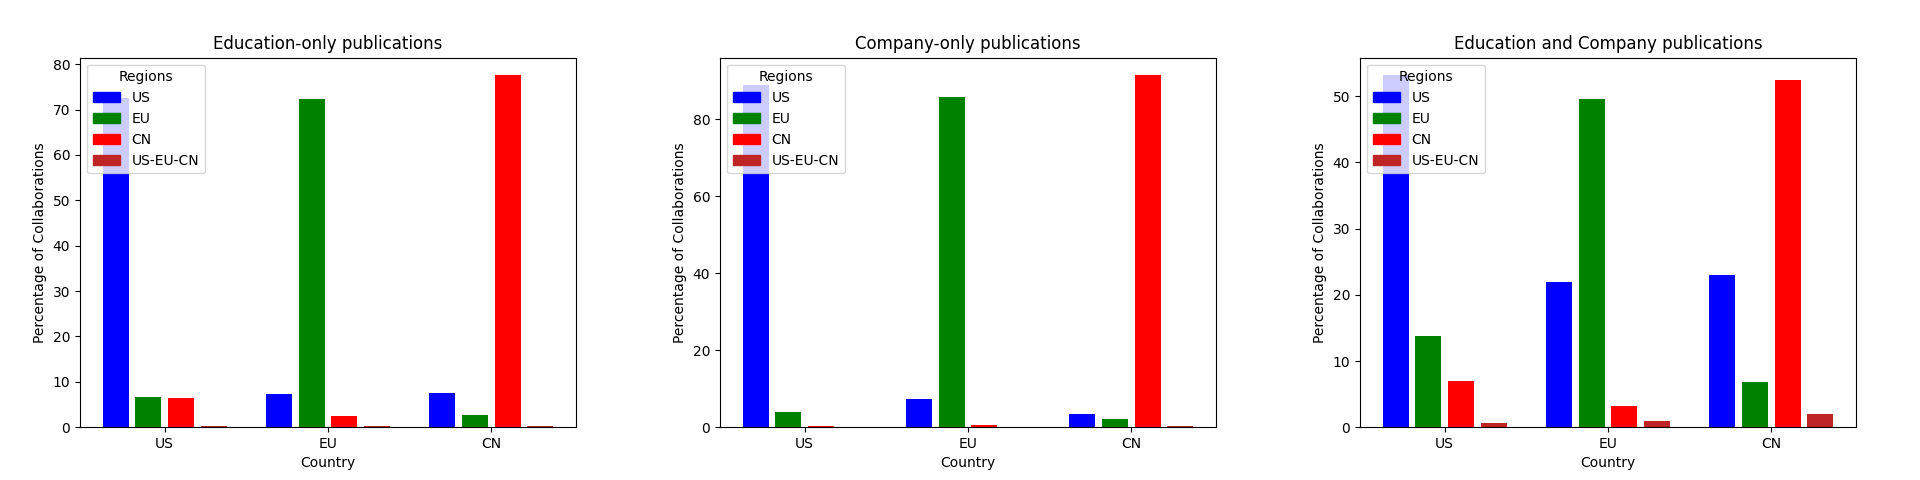
\includegraphics[width=0.8\textwidth]{images/collaboration_percentage_by_collab_type.png}
    \caption{Collaboration percentage by collaboration type}
    \label{fig:collaboration_percentage_by_collab_type}
\end{figure}

In in Figure \ref{fig:collaboration_percentage_by_collab_type}, we can observe how the countries go from 77.56\%, 72.38\%, and 72.58\% of self-collaboration for China, the EU, and the US respectively in the case of education-only co-authorship to a rate of 52.48\%, 49.52\%, and 53.17\% in the case of collaborations between mixed institution types. In addition to this, the percentage of papers published in collaboration with institutions from the US increased either for China or the EU, going from 7.61\% and 7.35\% for China and the EU in the case of educational institutions only, to 23.04\% and 21.90\% in the cases of mixed institution types.

\begin{table}[]
        \centering
    \begin{tabular}{lcccc}
    \hline
    Country & With CN & With EU & With US & All 3 regions \\ \hline
    CN      & 76,75\% & 2,91\%  & 8,13\%  & 0,36\%        \\
    EU      & 2,57\%  & 71,15\% & 8,29\%  & 0,32\%        \\
    US      & 6,27\%  & 7,23\%  & 71,33\% & 0,28\%        \\
            &         &         &         &               \\ \hline
    \end{tabular}
    \caption{Relative collaboration rates per country}
    \label{table:collaboration_percentage}
    \end{table}

Although in a long-term perspective the EU and the US were the most productive regions in terms of the number of papers published, in Figure \ref{fig:collaborations_between_countries_per_year} we can observe that China became the most published country in 2017, followed by the EU and the US. Regarding the articles published in collaboration, the EU and the US used to be the most productive duple, but in 2014, China and the US surpassed the previous couple, becoming the two most productive publishers as we can see in Figure \ref{fig:collaborations_between_countries_per_year}. The number of co-authored articles between China and the EU has been also increasing, having a positive tendency, similar to the one noted during the last 5 years between China and the US. Finally, we can observe that the number of collaborations between the three territories has been also increasing, especially since 2015.

\begin{figure}[tb]
    \centering
    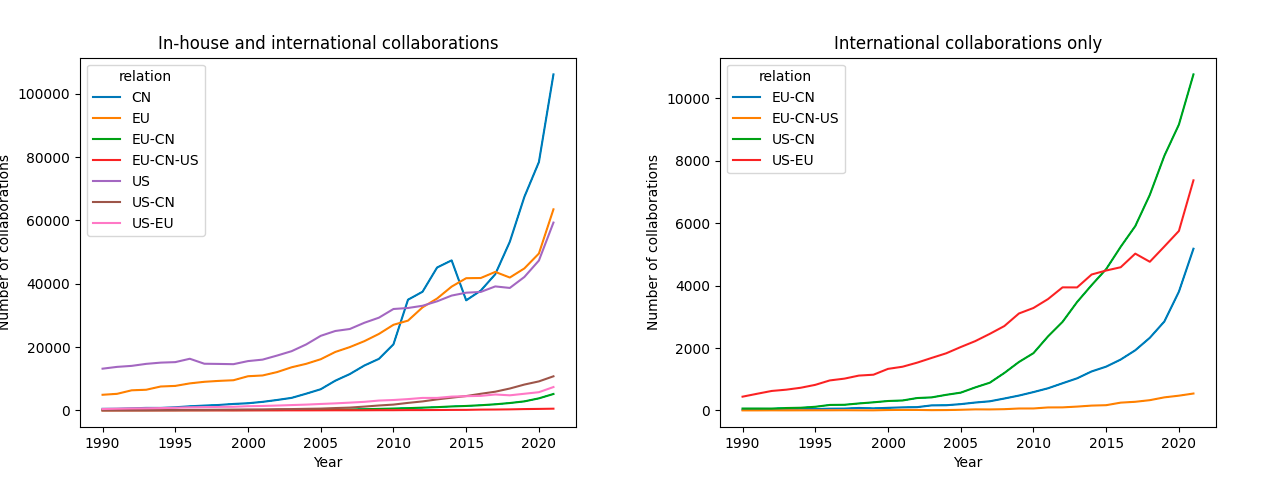
\includegraphics[width=0.8\textwidth]{images/collaborations_between_countries_per_year.png}
    \caption{Collaboration percentage by collaboration type}
    \label{fig:collaborations_between_countries_per_year}
\end{figure}

\subsection{Results for the Impact in research outcomes}

\begin{table}[]
    \centering
    \begin{tabular}{lcccccccc}
    \hline
    Collaboration type & CN-only & EU-Only & US-Only & CN-EU & CN-US & EU-US & CN-EU-US & AVG   \\ \hline
    All                & 13,32   & 21,64   & 37,24   & 24,14 & 27,89 & 38,12 & 32,88    & 27,89 \\
    Education          & 13,41   & 21,84   & 37,41   & 24,44 & 27,83 & 38,86 & 32,66    & 28,06 \\
    Company            & 6,41    & 15,4    & 31,95   & 19,59 & 15,87 & 17,8  & 11,11    & 16,88 \\
    Mixed              & 11,43   & 20,56   & 38,04   & 21,04 & 28,64 & 36,53 & 34,12    & 27,19 \\ \hline
    \end{tabular}
\caption{Average number of citations per collaboration type}
\label{table:avg_citations_by_collab_type}
\end{table}

Apart from the articles themselves, we have measured the number of citations as the outcome of the published articles. In an overall comparison, we found that the papers published through the collaboration between the EU and the US obtained the highest citation rate with an average of 38.12 citations per paper as we can see in Table \textit{\ref{table:table_avg_citations_by_collab_type}}. It´s followed by publications done by the US only with a 37.24 citation average, and by the publications where the three regions worked together with 32.88 average citations. The rest of the results are below an average of 30 citations per research paper, the least cited papers were those published only by Chinese institutions, with an average of 13.32 citations per paper, far from the second least cited publications, the EU only with an average of 21.64. However, China increased its rates by collaborating with the US and the EU, which also helped the EU to increase its own rates. Therefore, the collaboration between China and the US brought an average of 27.89 citations, as well as the collaboration between China and the EU brought an average of 24.14 citations, increasing their country-only rates for both regions, China and the EU. 
If we take a deeper look at the average number of citations between the actors across the different collaboration types, we see that those papers written by authors belonging to private companies had the least number of citations, with an average of 16.88, being China especially disadvantaged, with an average of 6,41 citations per paper, suggesting that publications from Chinese companies do not get relevance in academic research.

\begin{table}[]
    \centering
    \begin{tabular}{lcccccc}
    \hline
                       & CN         &                  & EU         &                  & US         &                  \\ \cline{2-7} 
    Collaboration type & \textit{r} & \textit{p-value} & \textit{r} & \textit{p-value} & \textit{r} & \textit{p-value} \\ \hline
    Education          & -0,18      & \textless{}.05   & -0,06      & \textless{}.05   & -0,01      & \textless{}.05   \\
    Company            & -0,14      & \textless{}.05   & 0          & 0,63             & 0,07       & \textless{}.05   \\
    Mixed              & -0,19      & \textless{}.05   & 0,01       & 0,04             & 0,08       & \textless{}.05   \\
    All                & -0,18      & \textless{}.05   & -0,06      & \textless{}.05   & 0          & \textless{}.05   \\ \hline
    \end{tabular}
\caption{Spearman Correlation Test results for the number of citations and the participation ratio per collaboration type}
\label{table:correlation_test_citations_participation_ratio}
\end{table}

We also analyzed how the number of participants from each region affect the final number of citations. To measure it, we compute the number of participants from a region over the total number of participants in the paper, obtaining a participation ratio. Then we used the Spearman Correlation Rank test to analyze if there is a correlation between the country participation ratios and the number of citations obtained. In Table \textit{\ref{table:table_table_correlation_test_citations_participation_ratio}}, we can see that the number of institutions from the US participating in the research article may not have an impact on the total number of citations. On the other hand, results suggest that there might be a weak negative correlation between the number of Chinese or European institutions participating in the research and the final number of citations. While for the UE, Spearman’s rank correlation between the two variables is -0.06 with a corresponding p-value of <0.05, for China this coefficient is three times higher, with a corresponding p-value of <0.05. Focusing on the different co-authorship types, we found that China had negative correlation values in all cases, the highest of those occurring in collaborations between Chinese companies and public institutions, where there was a negative correlation between the two variables, r (31641) = -0.19, p = <0.05. On the other hand, the EU had no significative correlation results in all cases but education, where it obtained a negative correlation of -0.06 with a corresponding p-value of <0.05. Finally, the US obtained positive correlation results in the collaborations between companies and between companies and public institutions, obtaining a positive correlation of -0.07 with a corresponding p-value of <0.05 and a positive correlation of -0.08 with a corresponding p-value of <0.05 respectively.

\subsection{Results for Researched Topics}

We have obtained the keywords of every publication, and we have listed the overall top 10 most used terms for every collaboration type between the regions. As we can see in Figure \ref{fig:topics_all_relations}, in China and the UE, as well as in their collaborations between them and the US, some topics have grown more than others. China seems to be prioritizing “Artificial Intelligence”, “Physics”, “Mathematics”, and “Engineering” over the others. Therefore, these topics have become the most published in internal collaborations, but China is also pushing these topics when working with international colleagues, raising these 4 topics in their collaborations with the EU and the US. Within these topics, the results suggest that China is particularly focusing on “Artificial Intelligence”, which is a topic that is being more researched in the last few years. Internal collaborations within the EU also have those 4 topics as the most researched. However, the EU is not only focusing on artificial intelligence. In contrast to the Chinese case, the EU patterns are not repeated when collaborating with the US, being in this case less grouped. The US does not have the clustering tendency we observed in the others. Although they are also researching more in “Artificial Intelligence”, it seems that they are also working on other fields such as “Psychology” or “Medicine”, relating them to the topic “Computer Science”. These topics are also observed when the US works with the EU, but not with China, suggesting that these are fields that may be more interesting for both.

\begin{figure}[tb]
    \centering
    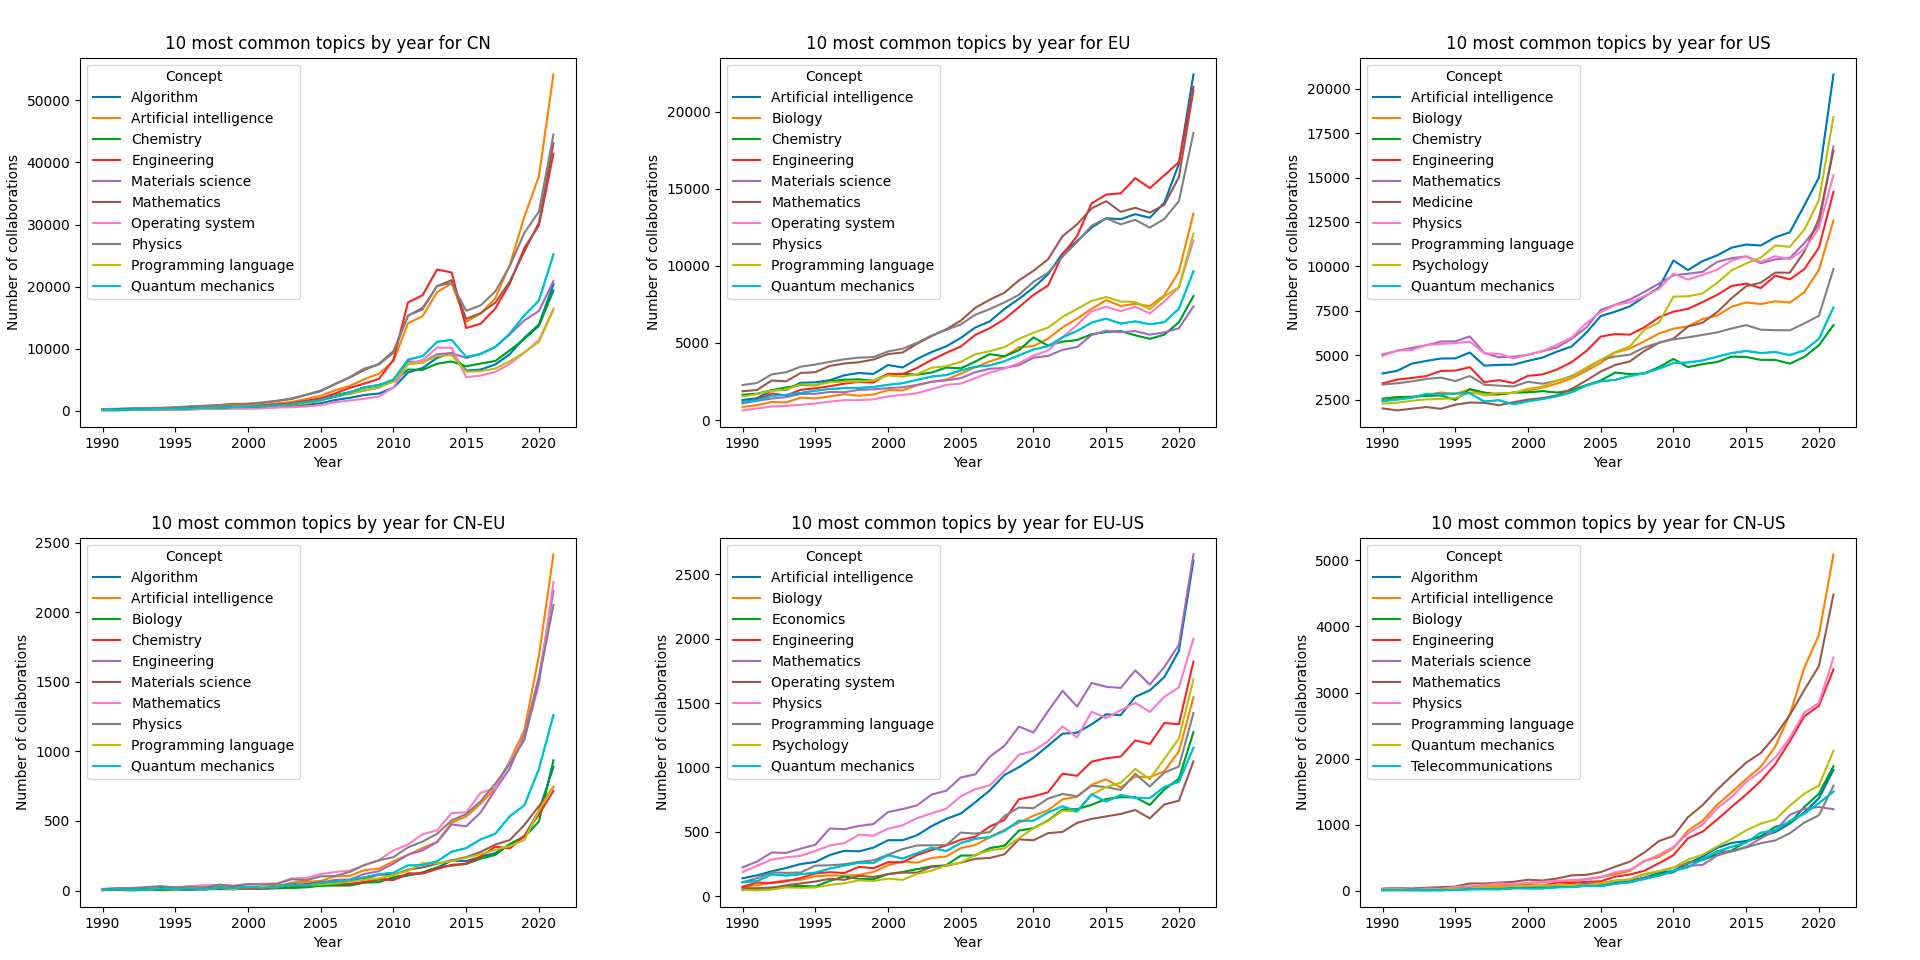
\includegraphics[width=0.8\textwidth]{images/topics_all_relations.png}
    \caption{Most researched topics by collaborating regions}
    \label{fig:topics_all_relations}
\end{figure}
\section{Conclusion}
\label{sec:conclusion}

In this study, we aimed to analyze the collaboration patterns and tendencies in the field of Computer Science for a long time, with special emphasis on China, the EU, and the US to provide a context on the status, benefits, and pitfalls for those collaborations.
First, we found that the US has been leading the research efforts in the field of Computer Science in the long term. However, it changed in recent years, when first China surpassed the US in 2011, only being exceeded by the US again in 2015, and second when the EU also surpassed the US in 2013. These results confirm the findings shared by the National Science Foundation placing China and the EU as the topmost productive regions in terms of number of publications in Science and Engineering \citep{burke2022state}. Because of this increase in Chinese publications, the number of co-authored articles between China and the US surpassed the previous leading collaborator partners, the EU and the US, in 2014. This change leaves China and the US as the top collaborators in Computer Science. Taking a deeper look into the different results obtained when analyzing the data based on the institution’s type that worked together, we observed that companies-only collaborations tend to be more internationalized, decreasing the number of self-collaborations only. This can be explained because the locations of headquarters or offices around the territories may help to increase the internationalization rate.
Second, we study the impact of the different regions when publishing their investigations, we found that those co-authored by the EU and the US tend to have the highest number of citations, suggesting that their findings tend to be more relevant than the others. In addition to this, results suggest that collaborating with the US also brings more citations for Chinese publications, obtaining twice as many as citations than the country obtains when publishing alone. These results, added that US-only papers obtained the second-highest average number of citations, indicate that the US has a big impact on their publications, either when the publication is alone or with institutions from other countries, which can be an important reason for the other countries to collaborate with the US. On the other hand, China and the EU benefit from collaboration between them too, both increasing their publication share when collaborating, compared to their works published when working within their countries only. Our results also indicate that articles published by Chinese companies were the least cited, suggesting that they might not be as relevant to other researchers as those published by colleagues from the EU or the US. In private sector collaborations, the US is clearly the most relevant, obtaining 39\% more citations on average than the second most cited, being those papers published by China and the EU.
Lastly, we found that China and the EU have been prioritizing “Artificial Intelligence”, “Physics”, “Mathematics”, and “Engineering” over others. This can also be seen when they have collaborated between themselves and the US. In contrast, the US has had not such a clear aim. Its research topics have been broader, including topics such as “Psychology” and “Medicine”. The EU has benefited from this wider approach by also collaborating with the US on these topics, bringing them more knowledge in the fields.
We can draw different conclusions for the three regions. First, while China produces the greatest number of scientific articles about Computer Science, their impact is relatively low. Hence, as observed in our study, China can benefit from collaborating with the EU and the US by obtaining more relevance in the scientific community and getting more quality in their publications. Its collaboration with the EU, whose interests seem to be aligned with China’s, can bring more, better, and more diversified studies for both partners. Apart from this, the EU can also take advantage of co-authorship with China by accessing the most productive region, in terms of the number of published papers. On the other hand, collaborating with the US can bring the EU high-quality knowledge about different topics, gaining more relevance in other fields. Lastly, the US can take advantage of collaborating with both China and the EU by accessing highly specialized research institutions, and in particular with the EU by creating high-impact publications, increasing the relevance of their institutions. Despite all these benefits for all the actors, politics can play a big role in collaborations between countries. Therefore, in future years, we will see which steps they decide to follow.
\section{Limitations and Future Work}
\label{sec:limitations}

In this study, only papers from OpenAlex were analyzed. Although is one of the largest databases, different results can be obtained when analyzing other sources.
Studying the status of funding and politics has not been the main aim of this study, although it has been reviewed. We know they play a main role in the relationship between countries, especially in partnerships. In future research, we would like to contribute current literature by these factors into current analysis and conclusions. 

\blankpage



% Anhang / Appendix
%\appendix % Ab hier wird mit A, B, ... weiternummeriert.
% Für den Fall eines Anhangs entkommentieren
%\section{Appendix}


% alle styles waren auskommentiert
%\bibliographystyle{WileyNJD-APA}%
%\bibliographystyle{acm}

\bibliography{references}

\end{document}